\section{Diskussion}
\subsection{Survey-modulet}
\begin{frame}{Modul forbedringer}
\begin{itemize}
\item Manglende besvarelse\\
\begin{tabular}{|l|l|l|}\cline{2-3}
\multicolumn{1}{l|}{} & Aktiv & Passiv\\\hline
Udsættelse & & \\\hline
Udeladelse & & \\\hline
\end{tabular}
\end{itemize}
\begin{itemize}
\item Tidspunkt for spørgsmål
\begin{itemize}
\item Reduktion \& Variation
\end{itemize}
\item Brugergrænseflade
\begin{itemize}
\item Dagbog
\end{itemize}
\end{itemize}
\end{frame}

\begin{frame}{Ikke-eksperimentiel}
Information fra survey-modulet kan anvendes som datakilde på lige fod med andre datakilder.
Dette lader patienten følge udviklingen i egne besvarelser af fx:
\begin{itemize}
\pause
\item Dagbog
\begin{itemize}
\item Daglige besvarelser
\item Ikke analytisk
\end{itemize}
\pause
\item Stemningsleje\\
{
\definecolor{fom}{RGB}{0,153,139}
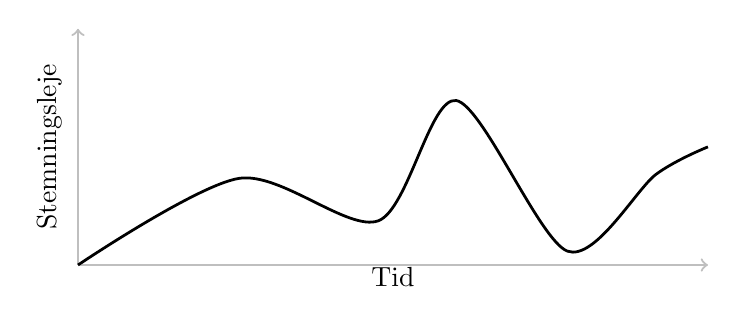
\begin{tikzpicture}[x=8cm,y=3cm]
\draw[thick, lightgray, ->] (0,0) -- (0,1);
\draw[thick, lightgray, ->] (0,0) -- (1,0);

%\draw [line width=1pt, lightgray] plot coordinates {(0,0) (0.2563,0.367) (0.4765,0.1869) (0.6004,0.6964) (0.777,0.0586) (0.9176,0.3838) (1,0.5)};
\draw [line width=1pt] plot [smooth] coordinates {(0,0) (0.2563,0.367) (0.4765,0.1869) (0.6004,0.6964) (0.777,0.0586) (0.9176,0.3838) (1,0.5)};
 
\node[label={[label distance=0.0cm,text depth=-1ex]center:Tid}] at (0.5,-0.05) {};
\node[label={[label distance=0.0cm,text depth=-1ex,rotate=90]center:Stemningsleje}] at (-0.05,0.5) {};
\end{tikzpicture}
}
\end{itemize}
\end{frame}

\subsection{Eksperimenter}
\newcommand{\mygraph}[2]{\definecolor{fom}{RGB}{0,153,139}
\begin{tikzpicture}[x=8cm,y=4cm]
\draw[thick, lightgray, ->] (0,0) -- (0,1);
\draw[thick, lightgray, ->] (0,0) -- (1,0);

\coordinate (end1) at (1.0,0.4321);
\coordinate (end2) at (1.0,0.5507) {};

\draw [line width=1pt, magenta] plot [smooth] coordinates {(0,0) (0.2563,0.367) (0.4765,0.1869) (0.6004,0.6964) (0.777,0.0586) (0.9044,0.3222) (end1)};
\draw [line width=1pt, fom] plot [smooth] coordinates {(0,0) (0.2325,0.2839) (0.4604,0.2355) (0.6001,0.7629) (0.7638,0.0278) (0.8912,0.4276) (end2)};
 
 \node[anchor=west] at (end1) {#1};
 \node[anchor=west] at (end2) {#2};
 
\node[label={[label distance=0.0cm,text depth=-1ex]center:Tid}] at (0.5,-0.05) {};
\end{tikzpicture}}
%(Sammenligning på tværs af sygdomme og Sammenligning på tværs af sensorer/analyser)

\begin{frame}{Social aktivitet}
\only<1>{\mygraph{SMS}{Sindst.}}
\only<2>{\mygraph{Opkald}{Sindst.}}
\only<3>{\mygraph{SMS}{Opkald}}
\only<4>{\mygraph{Social}{Sindst.}}
\end{frame}

\begin{frame}{Sammenligning med sygdom}
\only<1>{\mygraph{Depression}{Patient}}
\only<2>{\mygraph{Stress}{Patient}}
\end{frame}

\subsection{Validering}
\begin{frame}{Indsamling af data}
Data-kilder bør vurderes på følgende tre kriterier:
\begin{itemize}
\item Pålidelighed
\item Præcision
\item Frekvens
\end{itemize}
Begrænsninger i kilder kan kompenseres ved at kombinere flere kilder.
\end{frame}

\begin{frame}{Sindstilstand og social aktivitet}
Der findes ingen \textit{ground truth} til validering.
\begin{itemize}
\item Sindstilstand kan bestemmes af psykolog/psykiater
\begin{itemize}
\item Indsamlet information kan sammenholdes hermed.
\item Kontinuert indsamling $\rightarrow$ kontinuert udvikling.
\end{itemize}
\item Social aktivitet
\begin{itemize}
\item Ingen kendt skala.
\item Ingen kendt metode for fagfolk.
\item Bestemmes ved relation mellem forskellige kilder på social aktivitet.
\item Kontinuert indsamling $\rightarrow$ kontinuert udvikling.
\end{itemize}
\end{itemize}
\end{frame}

\subsection{Åbne problemstillinger}
\begin{frame}{Åbne problemstillinger}
Hvordan skal de indsamlede data analyseres?\\
Hvordan oplyser vi patienten, om de informationer der er i hæftet, på en mobil platform?\\
Hvordan præsenteres HAM-D på en mobil platform uden en interviewer?\\
Hvornår skal spørgsmål stilles for at få det bedste billede af patientens stemningsleje?\\

\end{frame}
